\subsection{Timing \& Synchronization}
\label{sec:fd-daq-timing}

\metainfo{David Cussans \& Kostas Manolopoulos.  This is an SP-specific section.  It's file is \texttt{far-detector-single-phase/chapter-fdsp-daq/design-timing.tex}}

%Describe the generation of timing/synchronisation signals and and distribution to the detectors.

All components of the DUNE \dword{sp} \dword{detmodule} are
synchronized to a common clock.  In order make full use of the
information from the \dword{pds} the common clock must be
aligned within a single \dword{detunit} with an accuracy of O(1ns).
In order to form a common trigger for \dword{snb} between
\dwords{detmodule} the timing between them must be aligned with an
accuracy of O(1ms).  However, a tighter constraint is the need to
calibrate the common clock to universal time (derived from GPS) in
order to adjust the data selection algorithm inside an accelerator
spill, which requires an absolute accuracy of O(1us).

Single and Dual phase detector modules use a different timing system,
driven by the different technical requirements and development history
of the two systems. A single phase detector module has many more
timing end-points than a dual phase module and many of the end-points
are simpler than the end-points in the dual phase, for example a \dword{wib}
vs. uTCA crate. Both systems have been sucessfully prototyped.

The DUNE \dword{sp} \dword{detmodule} uses a development of the protoDUNE
timing system. Synchronization messages are transmitted over a serial
data stream with the clock embedded in the data. The format is
described in DUNE DocDB-1651~\cite{docdb-1651}. Figurere~\ref{fig:daq-readout-timing}
shows the overall arrangement of components within the Single Phase
Timing System(SPTS). A stable master clock, disciplined with a \SI{10}{\MHz}
reference is used in the SPTS. A \dword{pps} is
also received by the system and is time-stamped onto a counter clocked
by the SPTS master clock, however the periodic synchronization
messages distributed to the \dword{sp} \dword{detmodule} are an exact number
of clock cycles apart even if there is jitter in the \dword{pps}.
%\fixme{Need reference added for DocDB-1651.}  done - ATH, 4/16/18

The GPS signal is encoded onto optical fibre and transmitted to the
CUC, where it is converted back to an RF signal on coaxial cable and
used as the input to a GPS displined oscillator. The oscillator module
also houses a IEEE 1588 (PTP) Grand Master and an NTP server. The PTP
Grand Master provides a timing signal for the \dword{dp} White Rabbit
timing network. The NTP server provides an absolute time for the
\dword{pps}. The SPTS relates its time counter onto GPS time by
timestamping the \dword{pps} onto the SPTS time counter and reading
the time in software from the NTP server.

The latency from the GPS antenna on the surface to the GPS receiver in
the CUC will be measured by optical time domain reflectometry at
installation. Given the modest absolute time accuracy required
(sufficient to select data within an accelerator spill) dynamic
monitoring of this delay is not required.

The White Rabbit synchronization signals from the \dword{dp} \dword{detmodule} are
time-stamped onto the SPTS clock domain and the SPTS synchronization
signals are time stamped onto the \dword{dp} clock domain. This allows
the timing in the \dword{sp} and \dword{dp} detectors to be
aligned. A similar scheme is used to relate the \dword{sp} protoDUNE
\dword{sp} timing domain to be related to the beam instrumentation
White Rabbit time domain.

In order to provide redundancy, and also the ability to easily detect
issues with the timing path, two independent GPS systems are used. One
with an antenna at the head of the Yates shaft, the other with an
antenna at the head of the Ross shaft. The two independent timing
paths are brought together in the same rack in the CUC. Using 1:2
fibre splitters one SPTS unit can be left as a hot-spare while the
other is active. This also allows testing of new firmware and software
during comissioning without the risk of loosing the SPTS if a bug is
introduced.


\begin{dunefigure}[Arrangement of Components in DUNE Timing System]{fig:daq-readout-timing}
  {Illustration of the components in the DUNE Timing System.}
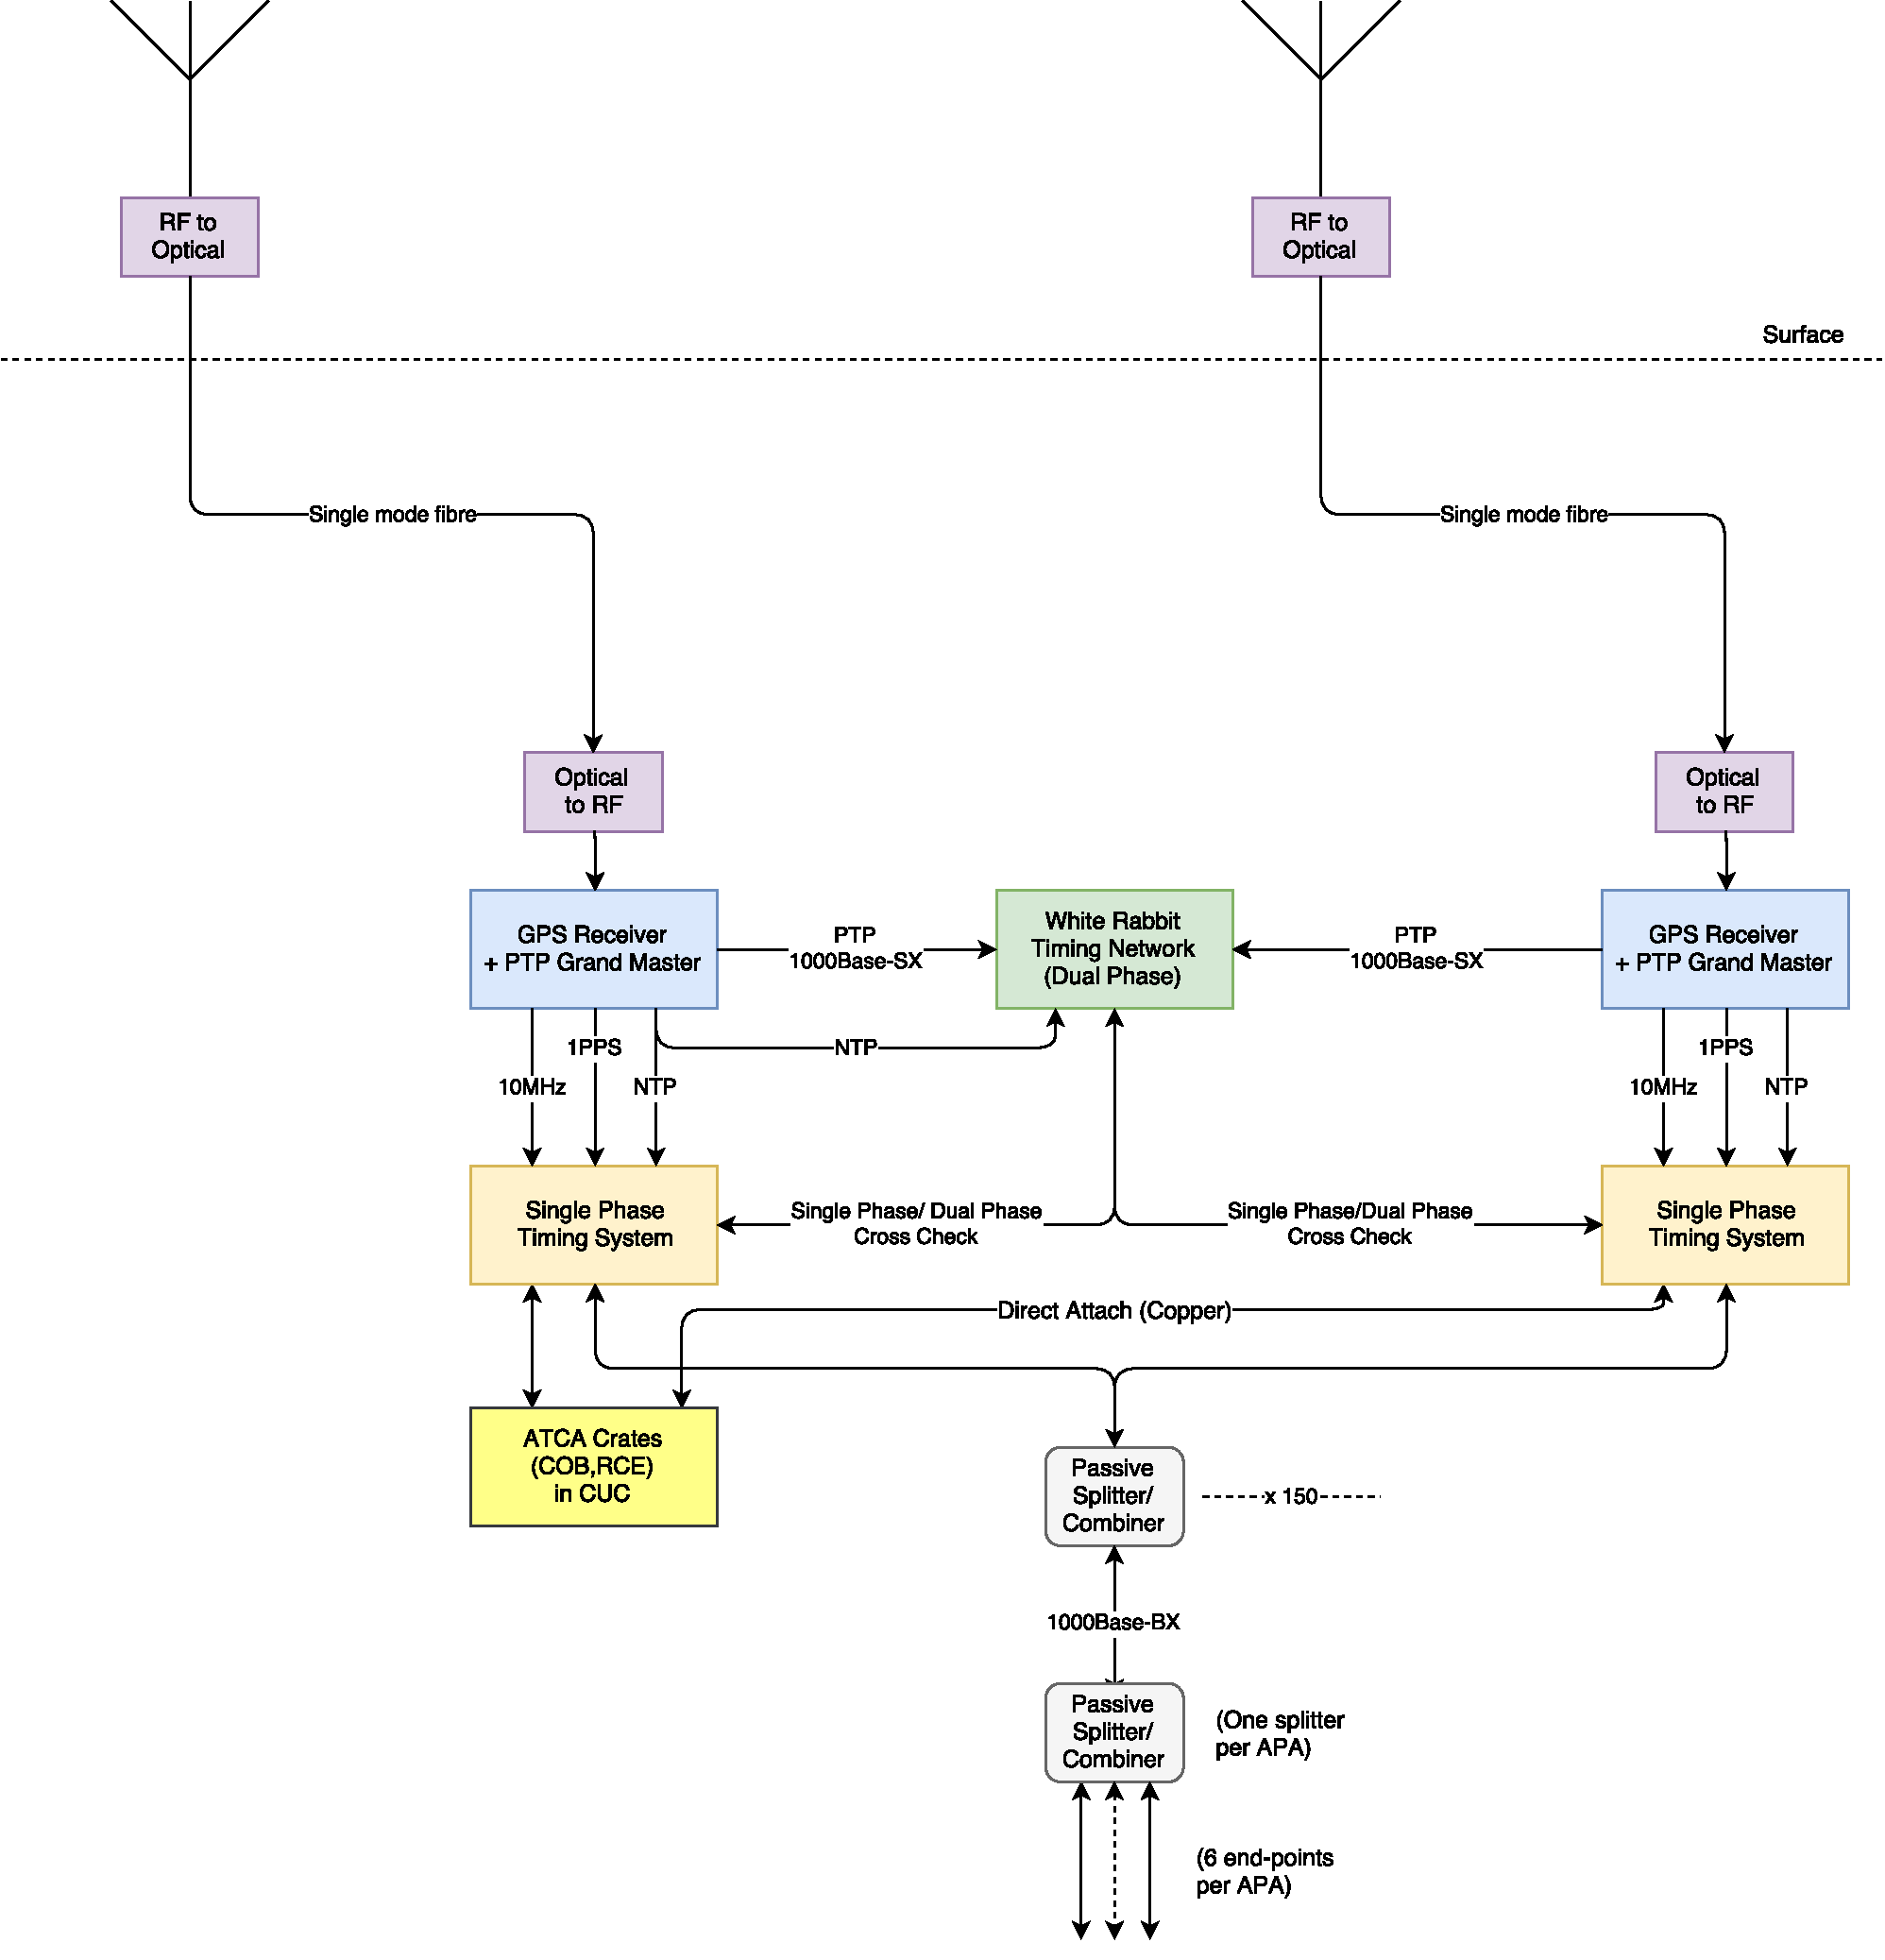
\includegraphics[width=0.8\textwidth]{DUNE_Timing_overall.pdf}
\end{dunefigure}

All the custom electronic components for the SPTS are contained in two
Micro-TCA shelves. At any one time one is active and the other is a
hot-spare. The \SI{10}{\MHz} reference clock and the \dword{pps} are received
by a single width AMC at the centre of the Micro-TCA shelf. This
master timing AMC produces the SPTS signals and encodes them onto a
serial data stream. This serial datastream is distributed over a
standard star-point backplane to the fanout AMCs which each drive the
signal onto up to 13 SFP cages. The SFP cages are either occupied by
1000Base-BX SFPs, each of which connects to a fibre running to an \dword{apa},
or to a Direct Attach cable which connects to systems elsewhere in the
CUC, {\it i.e.} the \dword{rce} crates and the data selection system. This
arrangement is shown in figure \ref{fig:daq-readout-sp-timing}


\begin{dunefigure}[Arrangement of components in \dlong{sp} timing system]{fig:daq-readout-sp-timing}
  {Illustration of the components in the Single Phase Timing System.}
  %\fixme{Add a diagram of the SPTS electronics}
  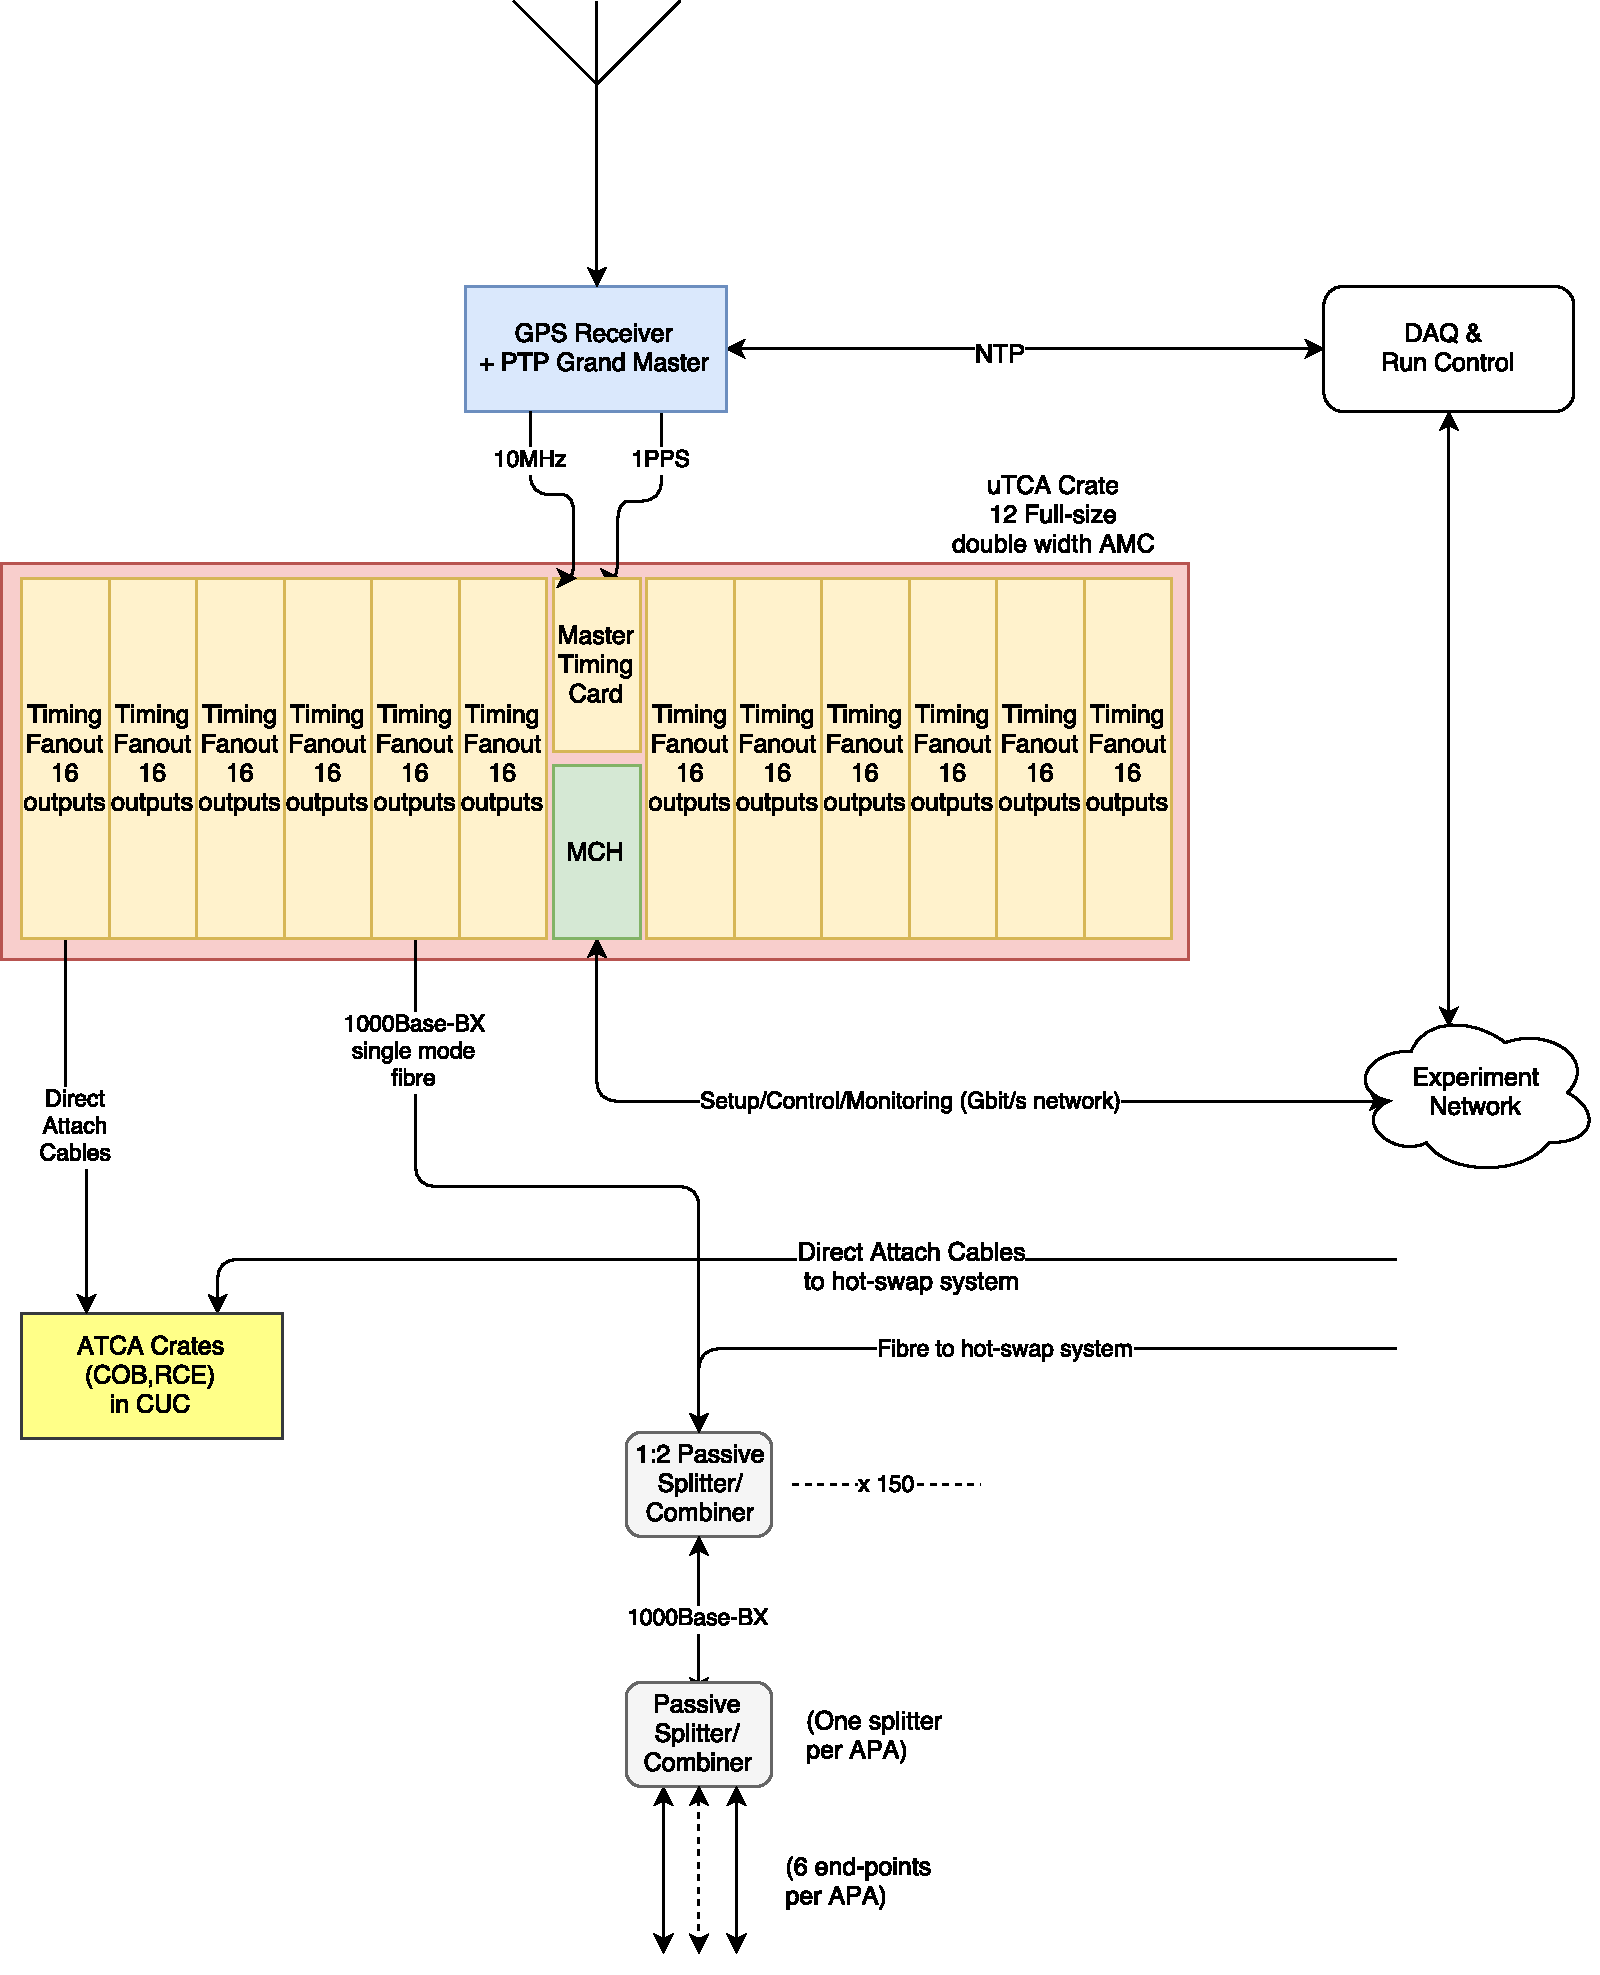
\includegraphics[width=0.8\textwidth]{DUNE_SP_Timing.pdf}
\end{dunefigure}



\subsubsection{Beam timing}
\label{sec:fd-daq-design-beamtiming}

The neutrino beam is produced at the Fermilab accelerator complex in
spills of \SI{10}{\us} duration. 
A \dword{sls} at the far detector site will locate the time periods in
the data when beam could be present, based on network packets received
from Fermilab containing predictions of the GPS-time of spills soon to
occur or absolute time stamps of spills recently occurring. 
Experience from MINOS and \nova shows that this can provide beam
triggering with high reliability with some small fraction of late or
dropped packets.
To improve further the system outlined here contains an extra layer
of redundancy in the prediction process. 
Several stages prediction based on recent spill behavior will be applied aiming
for an accuracy of better than 10\% of a readout
time (sub-\si{\ms}) in time for the data to be selected from
the \dword{daq} buffers. 
Ultimately, an offline database will match the actual time of the
spill with the data, thus removing any reliance on real-time network
transfer for this crucial stage of the oscillation measurements. The
network transfer of spill-timing information is simply to ensure a
correctly located and sufficiently wide window of data is considered
as beam data. This system is not required, and is not designed to
provide signals accurate enough to measure neutrino time-of-flight.

The precision to which the spill time can be predicted at \fnal
improves as the acceleration process of the protons producing the
spill in question advances.  The spills currently occur at intervals
of \SI{1.3}{\s}; the system will be designed to work with any interval, and
to be adaptable in case the sequence described here changes.  For
redundancy, three packets will be sent to the far detector for each
spill.  The first is approximately \SI{1.6}{\s} before the spill-time, which
is at the point where a \SI{15}{\Hz} booster cycle is selected; from this
point on, there will be a fixed number of booster cycles until the
neutrinos and the time is subject to a few ms of jitter.  The second
is about \SI{0.7}{\s} before the spill, at the point where the main injector
acceleration is no longer coupled to the booster timing; this is
governed by a crystal oscillator and so has a few \si{\us} of jitter.
The third will be at the so called `\texttt{\$74}' signal generated before the beam line kicker magnet fires
to direct the protons at the LBNF target; this doesn't improve the
timing at the far detector much, but serves as a cross check for
missing packets.  This system is enhanced compared to that of
MINOS-\nova, which only use the third of the above timing signals.  The
reason for the larger uncertainty in the time interval from \SI{1.6}{\s} to
\SI{0.7}{\s} is that the booster cycle time is synchronised to the
electricity supply company's \SI{60}{\Hz} which has a variation of about
1\%.

Arrival-time monitoring information from a year of MINOS data-taking
was analysed, and it was found that 97\% of packets arrived within
\SI{100}{\ms} of being sent and 99.88\% within \SI{300}{\ms}.

The \dword{sls} will therefore have estimators of the GPS-times of
future spills, and recent spills with associated data contained in the
\dwords{daqbuf}. These estimators will improve in precision as
more packets arrive.  The \dword{daq} will use data in a wider window than
usual, if, at the time the trigger decision has to be made, the
precision is less accurate due to missing or late packets.  From the
MINOS monitoting analysis, this will be very rare.


